\documentclass{article}[11]
\usepackage{palatino}
\usepackage{graphicx}
\usepackage[colorinlistoftodos]{todonotes}
\usepackage{indentfirst}
\usepackage[]{blindtext}
\usepackage{wrapfig}


\usepackage{float}
\usepackage{graphicx}

\definecolor{dkgreen}{rgb}{0,0.6,0}
\definecolor{gray}{rgb}{0.5,0.5,0.5}
\definecolor{mauve}{rgb}{0.58,0,0.82}

\usepackage{listings}
\lstset{frame=tb,
  language=Java,
  aboveskip=3mm,
  belowskip=3mm,
  showstringspaces=false,
  columns=flexible,
  basicstyle={\small\ttfamily},
  numbers=none,
  numberstyle=\tiny\color{gray},
  keywordstyle=\color{blue},
  commentstyle=\color{dkgreen},
  stringstyle=\color{mauve},
  breaklines=true,
  breakatwhitespace=true,
  keywordsprefix={@},
  tabsize=3
}

\usepackage{pdfpages}
%margins as described in "Ghid de redactare Diploma Licenta" by  Mihai Micea
\usepackage[top=1.37in, bottom=1.18in, left=1.18in, right=0.78in]{geometry}

\usepackage[english]{babel}
\usepackage{combelow}
\usepackage[utf8x]{inputenc}

%\useshorthands{'}
%\defineshorthand{'s}{\cb{s}}
%\defineshorthand{'a}{ă}
%\defineshorthand{'t}{\cb{t}}
%\defineshorthand{'S}{\cb{S}}
%\defineshorthand{'T}{\cb{T}}

\usepackage{acro}
\acsetup{first-style=short}

\DeclareAcronym{app}{
	short = app,
	long = application,
	class = abbrev
}

\DeclareAcronym{apps}{
	short = apps,
	long = applications,
	class = abbrev
}

\DeclareAcronym{SDM}{
	short = SDM,
	long = Software Design Methods,
	class = abbrev
}

\DeclareAcronym{OOD}{
	short = OOD,
	long = Object-oriented design,
	class = abbrev
}

\DeclareAcronym{UML}{
	short = UML,
	long = Unified Modeling Language,
	class = abbrev
}

\DeclareAcronym{DP}{
	short = DP,
	long = Design Patterns,
	class = abbrev
}

\DeclareAcronym{OOP}{
	short = OOP,
	long = Object-oriented programming,
	class = abbrev
}

\DeclareAcronym{MVP}{
	short = MVP,
	long = Model View Presenter,
	class = abbrev
}

\usepackage{hyperref}
\hypersetup{
    colorlinks=true,
    linkcolor=blue,
    filecolor=magenta,      
    urlcolor=cyan,
    citecolor=blue}

\begin{document}



\begin{titlepage}

\newcommand{\HRule}{\rule{\linewidth}{0.5mm}} % Defines a new command for the horizontal lines, change thickness here

\center % Center everything on the page
 
%----------------------------------------------------------------------------------------
%	HEADING SECTIONS
%----------------------------------------------------------------------------------------

\textsc{\LARGE Universitatea "Politehnica" Timi\cb{s}oara}\\[1.5cm] % Name of your university/college
\textsc{\Large Course: Software Project Management}\\[0.5cm] % Major heading such as course name

\vspace{3cm}


%----------------------------------------------------------------------------------------
%	TITLE SECTION
%----------------------------------------------------------------------------------------

\HRule \\[0.4cm]
{ \huge \bfseries %
		HelpMeSee\\ \Large
		Mobile personal assistant application for visually impaired people\\
		Project: Software Design Methods
}\\[0.4cm] % Title of your document
\HRule \\[1.5cm]
 
%----------------------------------------------------------------------------------------
%	AUTHOR SECTION
%----------------------------------------------------------------------------------------

\begin{minipage}{0.4\textwidth}
\begin{flushleft} \large
\emph{Author:}\\
Marius \textsc{Olariu} % Your name
\end{flushleft}
\end{minipage}
~
\begin{minipage}{0.4\textwidth}
\begin{flushright} \large
\emph{Lecturer:\hspace{2cm}} \\
Dr. Răzvan \textsc{Cioargă} % Supervisor's Name
\end{flushright}
\end{minipage}\\[2cm]

% If you don't want a supervisor, uncomment the two lines below and remove the section above
%\Large \emph{Author:}\\
%John \textsc{Smith}\\[3cm] % Your name

%----------------------------------------------------------------------------------------
%	DATE SECTION
%----------------------------------------------------------------------------------------



%----------------------------------------------------------------------------------------
%	LOGO SECTION
%----------------------------------------------------------------------------------------
\vspace{3.5cm}


\includegraphics{./imgs/UptLogo.jpg}\\[1cm] % Include a department/university logo - this will require the graphicx package
 
%----------------------------------------------------------------------------------------

\vfill % Fill the rest of the page with whitespace

\end{titlepage}

\tableofcontents
\newpage

\section{Description of the project}
	Nowadays software runs the world but most of the software solutions are designed for healthy people. Thus,  the visually impaired people are somehow left aside. However, recently things have begun to change and since everyone now owns a smartphone, there have been developed a series of apps for the visually impaired people. Most successful apps are \emph{Be My Eyes} (establishes a live video connection with an volunteer that describes the surroundings to the blind person), BeSpecular(the visually impaired person takes a photo, attaches a voice message to it and sends it to a volunteer that provides help) or the most helpful (in my opinion) \emph{Seeing Ai} from Microsoft. The later \ac{app} is an assistant which is able to recognize "saved" persons and describe their emotions, read text aloud from labels/books etc., provide description of images from other \ac{apps} (e.g. Facebook) by importing them into \emph{Seeing Ai} or scene description. However, it is developed only for \emph{iOS}. Apart from these, there are a variety of mobile assistan apps for the visually impaired people but most of them  have a free and limited variant and in order to make use of all the features the user has to purchase it. \\
	
	To address the issue with apps that need to be purchased and taking into account that the visually impaired people are in general in need of money (unless you are Andreea Bocelli) an free mobile assistant app will be developed, namely \emph{HelpMeSee}. This app  will offer a different perspective compared to what is on the market at this point. To achieve the aforementioned objectives\emph{HelpMeSee} will make use of cyber-foraging ("a technique to enable mobile devices to extend their computing power" \cite{lewis2016decision})) using the cloud resources provided by Google or Microsoft. We prefer to use these solutions because they are the work of more experienced developers and the purpose is not to  "reinvent the wheel" (e.g. implement proper variants of speech recognition, extracting a description from an image etc.). Also, cyber-foraging has the proven benefits: extends the computing power, saves storage space and extends battery life of mobile devices.

	%TODO add logo of the app
	%TODO  as motivation, add the benefits of cyber-foraging	
	
	\newpage

\section{Requirements}

\subsection{Functional requirements}

\subsubsection{Directions}
	The app should provide assistance to the blind user when he/she tries to get to a location. The user will be guided using voice instructions (e.g. "Go straight 100 meters", "You are about to cross the street").
	
\subsubsection{Location}
	The user can ask the app to retrieve his current location (e.g. "Bld. Industriei, nr. 6) and has the possibility to share his current location to a list of predefined friends.
	
\subsubsection{Scene description}
	By taking a photo the user is able to obtain information about his/her surroundings (e.g. "A red car is parked in front of you.") and this phrase will be read out loud.
	
\subsubsection{Text recognition}
	The app should be able to recognize text and read it out loud. The sources of text could be: text written on paper, labels on products or handwritten notes.
	
	
\subsection{Nonfunctional requirements}

\subsubsection{Usability}
	There must be designed mechanisms that allow the users to navigate through app and access its features easily given their condition.

\subsubsection{Maintainability}
	Due to the fact that bugs are inevitable the implementation of the app must adhere to \textbf{O}bject \textbf{O}riented \textbf{D}esign \textbf{P}rinciples (e.g. \textbf{S}ingle Class Responsibility, \textbf{O}pen-close, \textbf{L}iskov substitution, \textbf{I}nterface segregation, \textbf{D}ependency inversion - SOLID) and goals (loose coupling, high cohesion) so that the time spent fixing bugs will be reduced. 


\subsubsection{Extensibility}
	Based on the feedback received from users the app can be extended easily with new features without great effort. Thus, the architecture of the app must be chosen carefully.


\section{Specifications}

\subsection{Directions}
	In order to implement this feature the app will use \emph{Google Directions API} that will provide the fastest walking route from A to B. The fastest route is provided in json file having a certain format. The user is notified from 20 to 20m with spoken instructions about the itinerary.

\subsection{Location}
	Again, \emph{Google Directions API} and the \textbf{G}lobal \textbf{P}ositioning \textbf{S}ystem (GPS) of the phone will be used to retrieve the location of the user. The location is displayed on the phone and read aloud. Also, using the voice command "friends" the app will send user's location to a list of predefined friends using the \textbf{S}hort \textbf{M}essaging \textbf{S}ervice(SMS). To add a friend in this list the user should use the voice command "add friend" followed by the name of the friend. If the user can not be found in the contact list then the user is asked to provide his/her phone number.
	
\subsection{Scene description}
	\emph{Microsoft Cognitive Services} provides \emph{Computer Vision API} that can be used to distil actionable information from images. Therefore, the user takes a photo and then the app will communicate using \textbf{Re}presentational \textbf{S}tate \textbf{T}ransfer (REST) with Microsoft cloud services, namely to get a meaningful description from an image.
	
\subsection{Text recognition}
	The same Microsoft cloud services can be used to detect and extract text from an image.
	
\subsection{Usability}
	Each screen of the app will have a button in the bottom-right corner, the \emph{processCommandButton} button (processes voice commands). Thus, the user has the possibility to access a feature without having to navigate between the back and forth screens. For example if the user is currently walking to a destination but at some point decides to get some information about surroundings he has to use the \emph{scene description} feature, thus will press the \emph{processCommandButton} button speak "Speech Description" and the according screen will be launched. In this manner the user is not forced to abandon one activity in order to perform another.\\
	
	The widget's size will be slightly bigger than for a normal app in order to facilitate the access to it. Also, for a simple \emph{tap} the widget name will be spoken out loud and for \emph{double-tap} the widget functionality will be accessed.

\subsection{Maintainability}
	There will be implemented a series of design patterns known for their  positive effect on this maintainability alongside good coding practices (e.g comments, descriptive attributes/methods/class names, reduced size methods etc.). The Factory Method will be used in order to reduce coupling between client classes (e.g. the ones that implement the business logic) and those which communicate with the cloud servers to provide services (product classes). \\
	
	For accessing each subsystem (i.e. directions, locations, scene description, text recognition) the Facade combined with Singleton pattern will be used. By doing so we do not need to reimplement the functionality of the  button (present in each screen), thus no code duplication. Also the Facade pattern will allow us to introduce the much desired decoupling between clients and products.
	
\subsection{Usability}
	The architecture for \emph{HelpMeSee} is going to be \textbf{M}odel \textbf{V}iew \textbf{P}resenter (MVP). All the data that needs to be persisted will be a part of the \emph{model}. A \emph{view} will contain just the mappings between the UI elements and the objects that control them (no logic is added, for example handling user input actions). The purpose of the a view(screen) is just to display data and notify the \emph{presenter} about user's actions. Next, each \emph{view} will have a presenter that will interact with the model in order to bring data to the view, modify the state of the model, apply UI logic and most important - implement the business logic .

 
\begin{figure}[H] 
	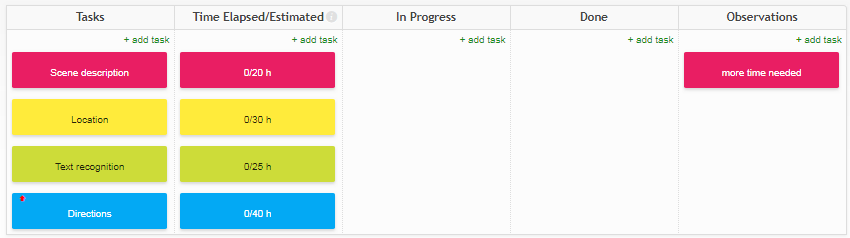
\includegraphics[width=16.5cm,height=8cm]{./imgs/taskSched}
	\caption{Tasks board}
\end{figure}

\section{Software Design Methods}
	\emph{\textbf{S}oftware \textbf{D}esign \textbf{M}ethods} (SPM) guide the software engineer in transforming the requirements into an executable software system. They offer theoretical foundations and at the same time some degree of freedom to innovate. However, there is no "silver bullet" \cite{brooks1987no} or one-size-fits-all for a complex software system.
According to Sommerville\cite{sommerville2010software} the \ac{SDM} can categorized in:

%TODO you can add more about reasons to use SDM to fill space SD-c8

	\begin{itemize}
		\item Top-down structured design
		\item Data-driven design
		\item \textbf{O}bject-\textbf{o}riented \textbf{d}esign (OOD)
	\end{itemize}

	Due to the fact that for this project we use an \textbf{O}bject-\textbf{O}riented paradigm for developing software we will discuss only the OOD methods applied for \emph{HelpMeSee}, that is:
	
	\begin{itemize}
		\item \textbf{U}nified \textbf{M}odeling \textbf{L}anguage (UML)
		\item  \textbf{D}esign \textbf{P}atterns (DP)
		\item \textbf{M}odel-\textbf{V}iew-\textbf{P}resenter (MVP) architecture
	\end{itemize}
	

\newpage

\subsection{Theoretical Background}

	\subsubsection{Model-View-Presenter}
	
	\begin{wrapfigure}{r}{0.6\textwidth}
		\centering
		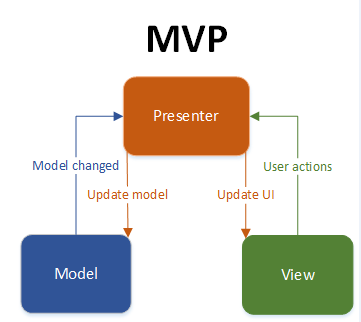
\includegraphics{./imgs/MVP}
		\caption{MVP architecture \cite{MVPPhoto}}
	\end{wrapfigure}
	
	 By using the \ac{MVP} architecture we maximize the code that can be tested with unit tests, separate business logic from UI (thus we adhere to OOP goals of low coupling, high cohesion or \emph{Single Responsability Principle}) and  end up with a codebase that is readable and maintainable.  This architecture is based on three types of classes: Model, View and Presenter. The \emph{Model} is responsible for the state of data, a \emph{View} for rendering UI elements and handling input/output from/to the user and the \emph{Presenter}  implements the business logic (moreover, works like a glue between the \emph{View} and \emph{Model}).\\
	
	 In particular for Android development, we will not end up with huge \emph{Activity} classes (they represent screens). Very often Android programming beginners end up with big Activity classes since there is not a clear distinction if such a class is an UI element or a business logic class, however, we will not detail further on this issue.
	
	\subsubsection{Unified Modeling Language}
	According to Martin Fowler \cite{fowler2004uml} \ac{UML} "is a family of graphical notations [...] that help in describing and designing software systems, particularly software systems built using the object-oriented (OO) style". From this family of diagrams we will be using only \emph{Class Diagrams}  and \emph{Use Cases}. Class Diagrams represent "the types of objects in system and the various [...] relationships that exist among them" \cite{fowler2004uml}. \emph{Use Cases} represent "a technique for capturing the functional requirements of the system"\cite{fowler2004uml} by using a graphical representation and  short instruction-like naratives (describe interactions of the users and system).

	\subsubsection{Design Patterns}
	Design patterns represent solutions to commonly occurring  problems when developing OO software systems. In other words, a DP is a template for how to solve a software development problem.
	\subsubsection{Facade}
	The \emph{Facade} pattern provides a high-level interface that eases the interaction with a complex subsystem. A real-life example of this pattern is when a client wants to place an order to a company (that does not have an online solution for this).  First, the client browses a catalogue to search for products codes/names. Next, client   calls a customer service representative (acts as a Facade) that register the order, creates the bill and gives the destination address to the shipping department. Coming back to the software domain, this pattern promotes decoupling between client and subsystem(s) but in the same time it does not prevent clients to interact directly with the subsystem. Facade pattern is often used in combination with the \emph{Singleton} pattern.
	
	\begin{figure}[H]
		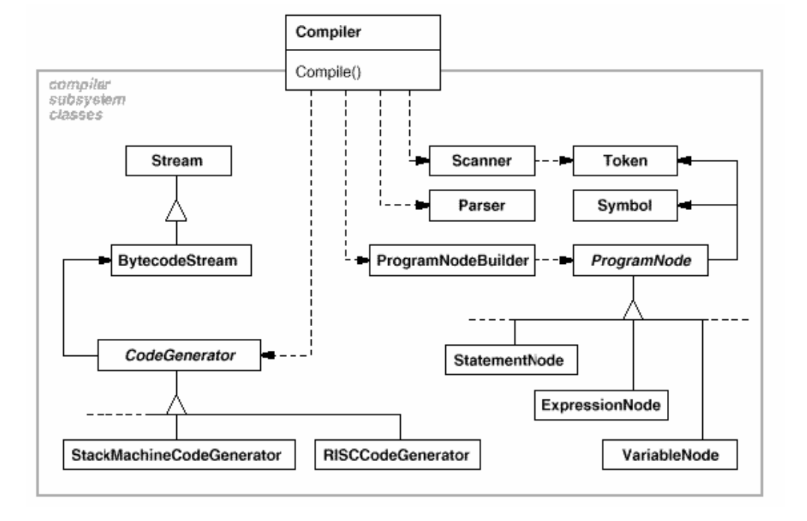
\includegraphics[scale=0.8]{./imgs/Facade}
		\caption{Example of applicability for Facade pattern  \cite{gamma1995design}}
	\end{figure}
	
	\subsubsection{Abstract Factory}
		Provides an interface for creating and managing families of objects without specifying their concrete classes \cite{gamma1995design}. For example when we design an app that has to change the look and feel of its GUI widgets according to user's preferences (the user can choose the look and feel at runtime). Although the GUI appearance will change, the functionality of widgets will remain the same. In the part of the code where the functionality of the widgets is implemented depends we would end up with a lot of \emph{ifs} that instantiate handle the concrete widget classes and more important with dependencies to that handle which widget classes. To solve the problem we could create an factory that would handle the widget instantiation and changing the widgets would mean just to change the factory that creates and retrieves them.\\
		By using this pattern we obtain independence on how products are created and represented, low coupling between clients and products. 
		\begin{figure}[H]
	
			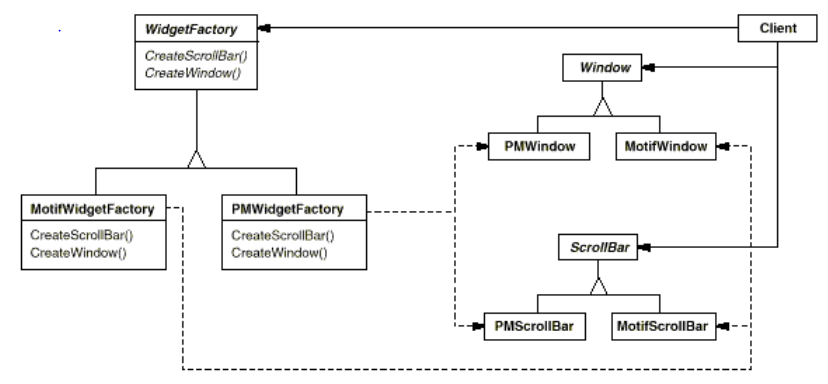
\includegraphics[scale=0.75]{./imgs/Factory}
			\caption{Example of applicability for Abstract Factory pattern \cite{gamma1995design}}
		\end{figure}
	\subsubsection{Singleton}
	By applying the Singleton pattern to a class we ensure that the respective class has only one instance and there is provided a global point of access to this instance. Often, in an app we need to have only one instance of a class, e.g. : the class that handles the connection to database, the class that handles the printing jobs, a window manager etc. . This pattern is often used in conjunction with other patterns like \emph{Abstract Facory} or \emph{Facade}.
	\begin{figure}[H]
		\centering
		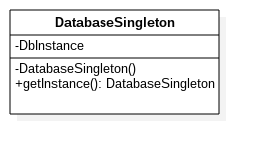
\includegraphics[scale=0.9]{./imgs/Singleton}
		\caption{Only one Database connection is needed per system}
	\end{figure}

\subsection{Concrete application of the SDM}
	Basically, the HelpMeSee app is centered around the navigation feature, i.e. helping the visually impaired person to get to  a certain destination, as can be seen in the \emph{Use Case} diagram too. Thus, the user can choose to use the \emph{Directions} feature and at any point in time to switch shortly to use another feature (while on his way to destination) using the \emph{processCommandButton} (present in every screen). By doing so we improve the usability of the app because the user does not have to quit his current activity (navigation) to get extra information about environment.

	\paragraph{HelpMeSee use cases:\\}
	
	
	\paragraph{Get to location B\\}
	
	\begin{enumerate}
		\item The user launches the \emph{Directions} screen from the \emph{Main-Menu} screen.
		\item The user provides destination location using text or voice input.
		\item The app renders the path to destination.
		\item The app notifies the user that everything is set-up and good to go.
		\item As user moves the app notifies him/her with voice instructions.
	\end{enumerate}
		
	\paragraph{Where am I?}

	\begin{enumerate}
		\item The user launches the \emph{Location} screen from \emph{Main-Menu} screen or through \emph{processCommandButton}.
		
		\item The app. displays user location on the screen and reads it out loud.
		
		\item The user can choose to send his location to a list of friends.
		\begin{enumerate}
			\item The user can add a new friend to the "friends list"
			\item The user can play again the reading of location by  tapping the half upper part of the screen twice.	
		\end{enumerate}
					

	\end{enumerate}			
	
	
	\paragraph{Text Detection}

		\begin{enumerate}
			\item The user launches the \emph{TextDetection} screen from \emph{Main-Menu} screen
			
			\item The app will start a timer of 5 seconds, when it expires it will take a photo
				\begin{enumerate}
					\item The user can take the photo before the timer expires using \emph{takePictureButton} 				
				
				\end{enumerate}
			
			\item The app reads loud the detected text
			
			\item User can take another photo or replay the previous detected text
						
		\end{enumerate}			
	
	\paragraph{Scene Description\\}
	
		The interactions between the system and the user are the same as with those described in the \emph{Text Detection} scenario. The only difference is represented by the backend algorithm that processes the photo.


	\includepdf[pages=2]{UML.pdf}


%\begin{figure}[H]
	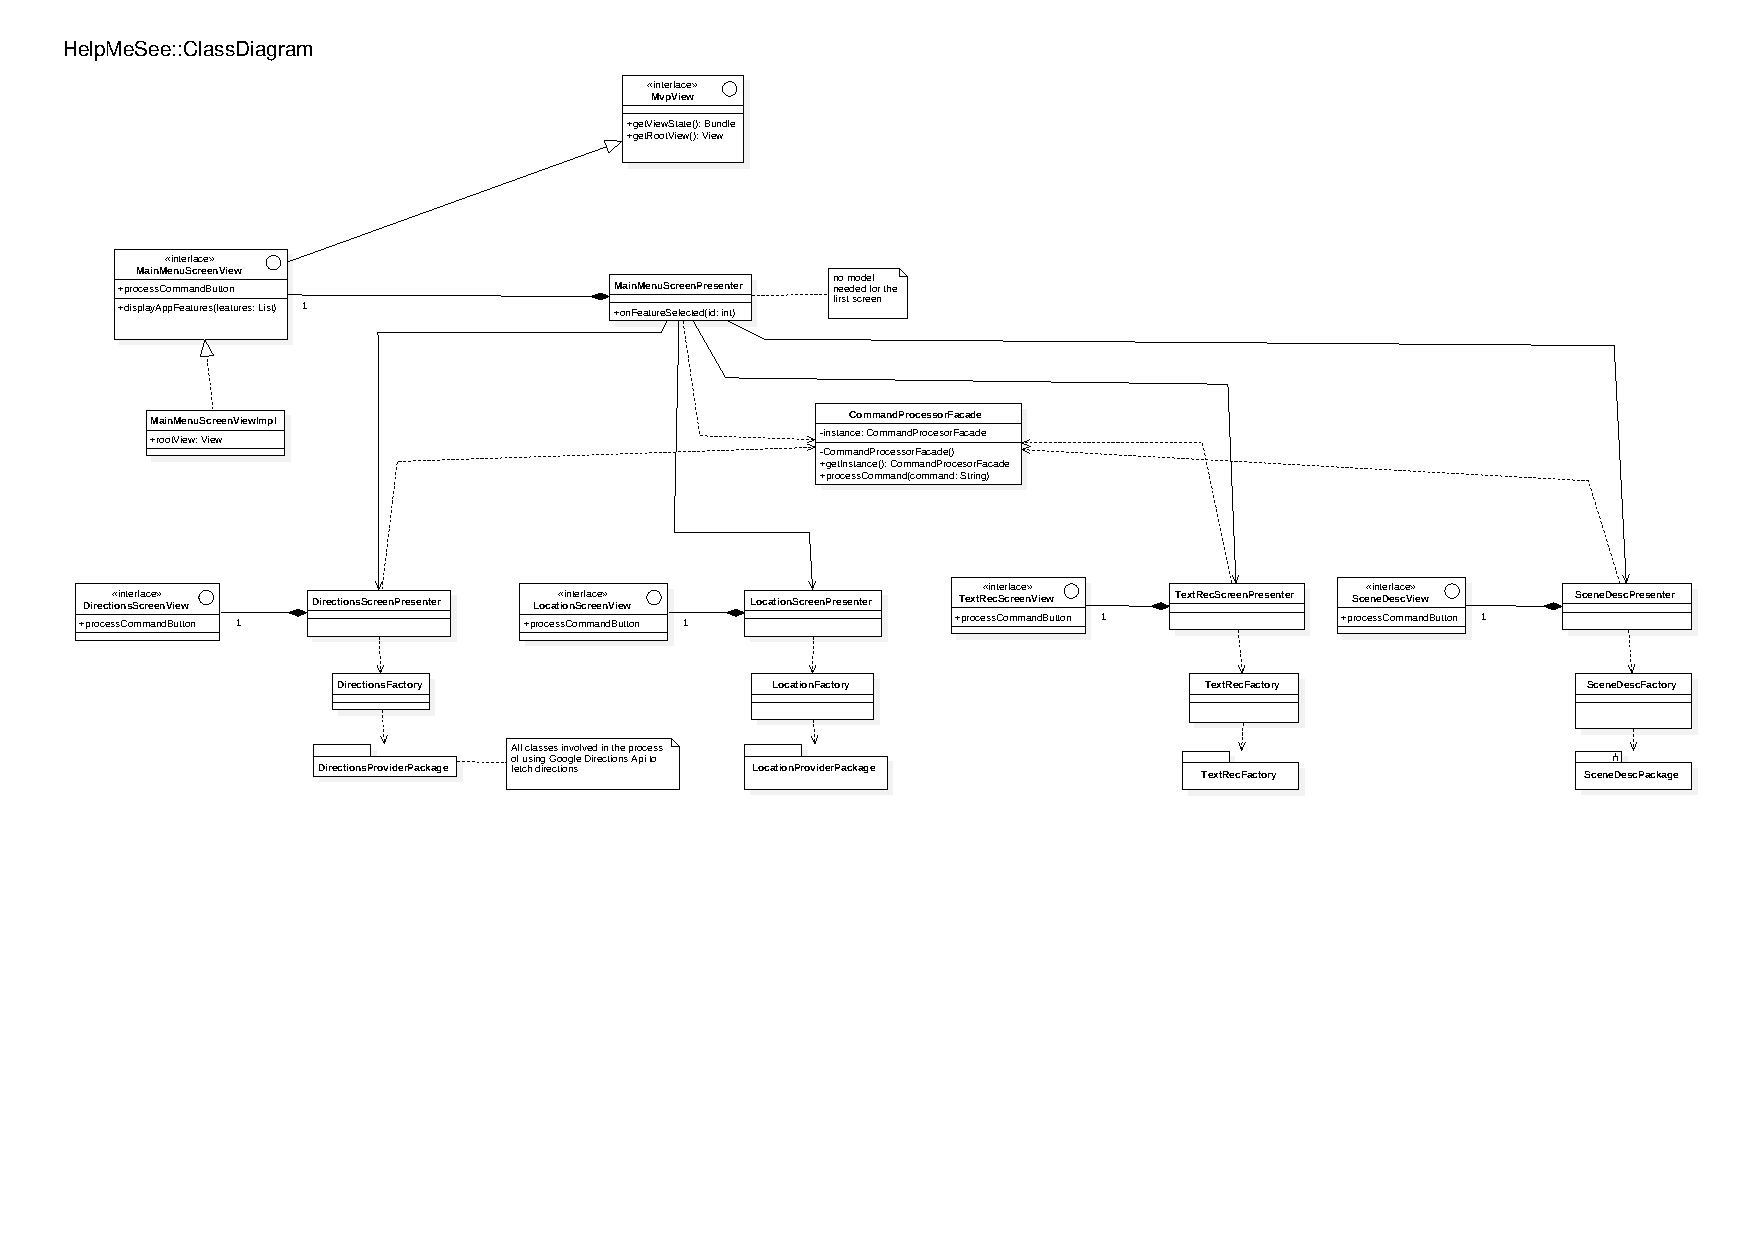
\includepdf[pages=1,angle=-90]{UML.pdf}
	%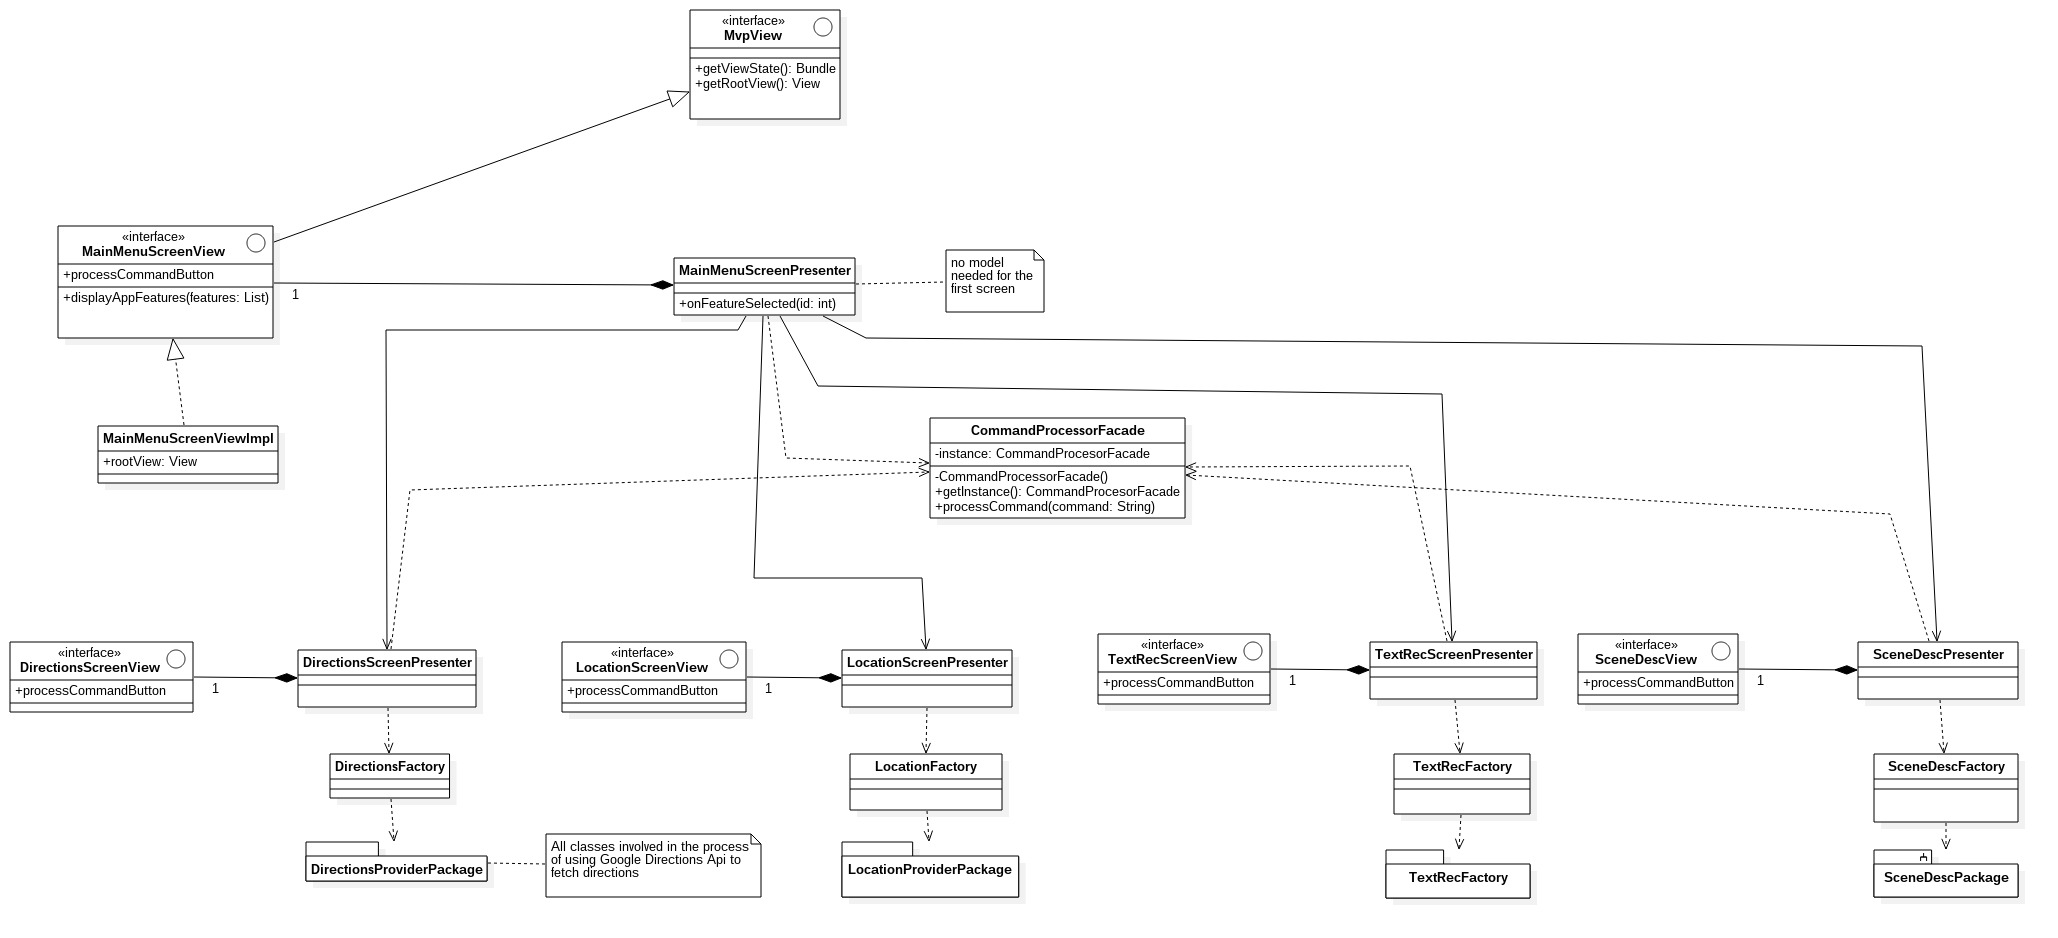
\includegraphics[scale=0.3, angle = -90]{./imgs/CD}
	%\caption{Class diagram of most important entities from HelpMeSee app}
%\end{figure}

 \paragraph{Model-View-Presenter\\}
 
 \subparagraph{Views\\}
 
   \emph{HelpMeSee} has 5 screens: \emph{Main-Menu}, \emph{Directions}, \emph{Locations}, \emph{Scene Description} and \emph{Text Recognition}. For each view there is defined a set of operations  that they need to handle, by implementing the following interfaces: \emph{MvpView}, \emph{\textbf{[ScreenName]}View} and \emph{\textbf{[ScreenName]}Listener} . For example, the \emph{Main-Menu} screen uses the following interfaces: \emph{MvpView}, \emph{MainMenuScreenView} and \emph{MainMenuScreenListener}. \\
   
   \emph{MvpView} defines the two services that all the screens need to provide, namely: \emph{getViewState():Bundle} (a mapping of key-value pairs that describe the properties displayed on the screen at a certain point in time, e.g the text displayed on some widget) and \emph{getRootView():View} (usually the parent layout for an Android screen). These two operations are necessary to each \emph{Presenter} to implement the logic and to update the screen if necessary. Next, \emph{\textbf{[ScreenName]}View} defines the particular operations that the screen needs to handle, for instance the \emph{MainMenuScreenView} interface contains only \emph{+displayAppFeatures(features:List)} method. For each screen the associate listener is the \emph{Presenter} (implements \emph{\textbf{[ScreenName]}Listener)} that contains the logic for handling a certain user input (the responsability is took out from the screen).\\
      
    As can be seen above, the only responsibilities of \emph{Main-Menu} screen is to display data provided by someone else (i.e the Presenter) and to pass the user interactions with the screen to the presenter. By doing so we respect the MVP architecture requirements for a View. This approach is repeated for the other screens too.
    
  \subparagraph{Presenters\\}
  	The purpose of presenters is to implement the business logic and since they are distinct for each screen there is no common interface. Moreover since no entity in the app depends on their interface (but rather, they depend on other entities) they are implemented as classes. As an example of presenter, the \emph{MainMenuPresenter} acts as bridge between the features that the app provides (entry point for using one of them). Consequently, the following snippet provides an overview of how the business logic that needs to be implemented.
  	
  	\begin{lstlisting}[caption = onFeatureSelected() mock]	
  	
  		public void onFeatureSelected(long id) {
    	final AppFeaturesEnum selectedFeature = AppFeaturesEnum.valueOf(appFeaturesList.get((int) id));

    	  //TODO : launch the selected feature
    	  switch (selectedFeature) {
      		case LOCATION:
        		Log.i(MAIN_SCREEN_TAG, "Launch Location screen");
        		break;

      		case DIRECTIONS:
       			Log.i(MAIN_SCREEN_TAG, "Launch DIRECTIONS screen");
        		break;

      		case SCENE_DESCRIPTION:
        		Log.i(MAIN_SCREEN_TAG, "Launch SCENE_DESCRIPTION screen");
        		break;

      		case TEXT_RECOGNITION:
        		Log.i(MAIN_SCREEN_TAG, "Launch TEXT_RECOGNITION screen");
        		break;
      
     		default:
        		Log.e(MAIN_SCREEN_TAG, "Feature doesn't exist!");
    	  }
  		}
  	\end{lstlisting}
  
  \subparagraph{Model\\}
  		For the moment the app does not need a proper model because the user never changes the state of the data (e.g. for instance it cannot change the directions for a certain route or change the text describing a scene in an image using user inputs).

  \paragraph{Facade\\}
  	As mentioned before in this document, in order to make the app more usable the user can give voice commands, these commands are for the moment the names of the features that the user wants to access: Location, Directions, Text Recognition, Scene Description. In each screen there will be the button \emph{processCommandButton} that will start the microphone for recording. After the command is decoded an action will be taken concordantly, e.g when on track to a destination user wants to obtain a "scene description" (it will launch \emph{SceneDescription} screen by pronouncing "scene description"). However, using this approach each presenter would end up "knowing" about the other features of the app (not to mention the duplicate code involved) and this would represent an escalation of the whole MVP architecture. In order to overcome this issue the \emph{Facade} pattern (implemented as a Singleton) is used having the following interface:
  	
  	\begin{figure}[H]
  		\centering
		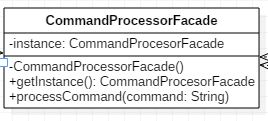
\includegraphics[scale=1]{./imgs/FacadeImpl}  	
  		\caption{Facade pattern concrete implementation}
  	\end{figure}
  	
  	Now, the button will pass only the voice command (e.g. "Location") to the \emph{Facade} that will handle the ease the access to features and solves the coupling problem aforementioned.
  	
  	\paragraph{Abstract Factory\\}
  	For each feature there is a package that provides the functionality. However, over it is not useful to instantiate over and over again the same objects or the clients to know about the specific classes that they need to instantiate. Therefore, an Abstract factory is defined for each package (e.g \emph{LocationFactory}, \emph{DirectionsFactory} etc, they can be seen in the UML diagram), and these factories will control and retrieve object instantiation for each class in a certain package. Also, they are implemented as singletons (since it doesn't make sense to have more than one factory per package) and will use a \emph{Object Pool} to retrieve the already created and reusable objects.
  	
  	\paragraph{Singleton\\}
  	Singleton is one of the simplest and most useful design pattern and for our project was used for the factory classes and \emph{CommandProcessorFacade} class.
    
\printacronyms[include-classes=abbrev,name=Abbreviations]



%the place where references will appear in output pdf
%good practice: bib name should be the same to the .tex file
\bibliography{SPMdoc}

%style
\bibliographystyle{ieeetran}


\end{document}